\chapter{Clusterização}
\label{cap:CLUSTERIZACAO}

Clusterização, ou ainda, análise de Cluster é a classificação não-supervisionada de padrões (sejam eles dados recolhidos, observações, ou ainda, vetores de atributos) em grupos concentrados chamados de \textit{Cluster}. Um exemplo de clusterização é apresentado na Figura \ref{fig:DATA-CLUSTERING}\cite{Jain:1999:DCR:331499.331504}, onde na Figura \ref{fig:DATA-CLUSTERING}(a) é apresentado o cojunto de informações de entrada e na Figura \ref{fig:DATA-CLUSTERING}(b) é apresentado o resultado de agrupamento dos dados analisados.

\begin{figure}[!h]
\centering 
\caption{Exemplo de Clusterização}
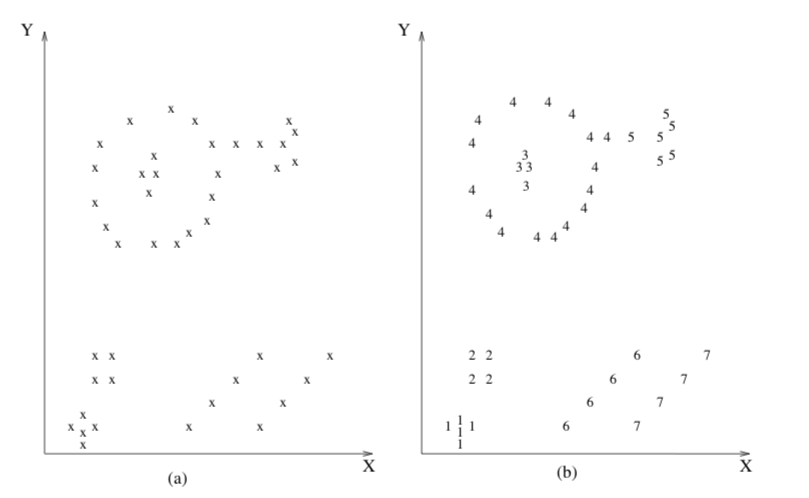
\includegraphics[width = \textwidth]{imagens/dataclustering.png}
\legend{Fonte: \citeauthor{Jain:1999:DCR:331499.331504}}
\label{fig:DATA-CLUSTERING}
\end{figure}

%A diferença entre clusterização (classificação não-supervisionada) e análise descriminante (classificação supervisionada) é que na segunda classificação os padrões estão rotulados 

Hoje a clusterização representa uma das principais etapas de análise de dados e é amplamente abordada em muitos contextos e por vários pesquisadores em suas disciplinas. Por conta do uso multidisciplinar e também a contextualização em diferentes comunidades, as metodologias, termos e até fases de implementação recebem nomes distintos da área de aplicação dos seus algoritmos.

A Clusterização é muito usada em análises exploratórias de padrão, agrupamento de dados, tomadas de decisão e muitas situações de \textit{Machine Learning} incluindo \textit{Data Mining}, recuperação de documentos, segmentação de imagens e classificação de padrões.

\section{Componentes de uma Tarefa de Clusterização}

A Clusterização tem esses passos como principais para o agrupamentos de objetos:
\begin{enumerate}
\item \textit{representação de padrões}: Fase em que se inclui, opcionalmente, a extração de atributos e ou extração de seleção. Aqui ocorre a a análise da classe, tipo, número e escala dos atributos que são importantes para o processo de clusterização. A seleção de atributos é a busca dos atributos mais efetivos e a extração de atributos é quando se faz necessário uma ou mais transformações dos atributos originais para gerar atributos mais notáveis para o \textit{clustering};

\item \textit{definição de uma medida de proximidade de padrões (sendo essa medida adequada aos dados observados)}: Fase que geralmente mede a distância entre pares de padrões. Para o cálculo simples entre dois atributos pode ser utilizada a distância Euclidiana. Já para outros cálculos de distância, outras fórmulas de distância são necessárias;

\item \textit{clusterização ou agrupamento}: Fase que pode ser desempenhada de varias formas. O agrupamento pode ser classificado como \textit{crisp} (onde cada padrão pertence ou não a um determinado grupo) ou \textit{fuzzy} (onde cada padrão pode apresentar graus de relacionamento com os grupos). Os algoritmos de clusterização hierárquica produz séries de partições aninhadas onde os objetos se unem ou se separam levando como critério a similaridade de seus atributos. Os algoritmos de clusterização particional identificam as melhores partições sendo otimizadas a cada iteração com base nos critérios de agrupamento.; 

\item \textit{apresentação dos resultados}: Fase que extrai os resultados da clusterização para uma linguagem simplificada e de fácil interpretação quando é um processo humano-orientado ou com atributos úteis e de melhor processamento quando é um processo automatizado;
\end{enumerate}

\begin{figure}[!h]
\centering 
\caption{Tarefas de Clusterização}
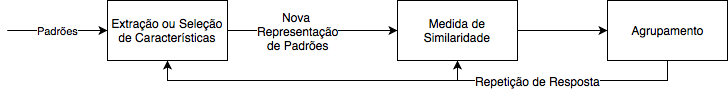
\includegraphics[width = \textwidth]{imagens/fasesclusterizacao.png}
\legend{Fonte: \citeauthor{Jain:1999:DCR:331499.331504}}
\label{fig:FASES-CLUSTERIZACAO}
\end{figure}

\newpage

\section{Definições e Notação}
Essa sessão tem o objetivo de apresentar as definições básicas e as notações que serão utilizadas nas sessões seguintes.

\begin{enumerate}
\item Padrão (ou ainda, vetor de atributos) \textbf{x} é um item único usado pelo algoritmo de clusterização. Geralmente é um vetor de $\mathit{d}$ medidas: $\mathbf{x}= (x_{1}, ..., x_{d})$.

\item O componente escalar $x_{i}$ do padrão \textbf{x} é chamado de característica ou atributo.

\item $\mathit{d}$ é chamado de dimensionalidade do padrão ou do espaço do padrão.

\item O conjunto padrão é denotado por $X= \left\{ \mathbf{x}_{1}, ...,\mathbf{x}_{n}\right\}$. O padrão $i$ em $X$ é denotado por $\mathbf{x_i}= (x_{i,1}, ..., x_{i,d})$. Há casos em que o conjunto padrão é uma matriz de padrões com as dimensões $n\times d$.

\item Classe é um estado que reflete características de um objeto e ou de um grupo com similaridades. Cada classe apresentada após o uso de uma técnica de clusterização reflete um grupo contido no conjunto padrão inicial da análise.

\item A técnica \textit{crisp} assume um rótulo de classe $l$ para cada padrão $\mathbf{x_i}$. O conjunto para todos os rótulos para um conjunto padrão $X$ é $L=\left\{l_1, ..., l_n\right\}$ com $l_i \in \left\{1, ..., k\right\}$, onde $k$ é o número de \textit{clusters}.

\item A técnica \textit{fuzzy} assume para cada padrão $\mathbf{x_i}$ uma fração $f_i,j$ que expressa o grau de associação em cada \textit{cluster} $j$.  
\end{enumerate}
